\documentclass[12pt,a4paper]{article}
%\usepackage{ctex}
\usepackage{amsmath,amscd,amsbsy,amssymb,latexsym,url,bm,amsthm}
\usepackage{epsfig,graphicx,subfigure}
\usepackage{enumitem,balance}
\usepackage{wrapfig}
\usepackage{mathrsfs, euscript}
\usepackage[usenames]{xcolor}
\usepackage{hyperref}
\usepackage[vlined,ruled,commentsnumbered,linesnumbered]{algorithm2e}
\usepackage{ulem}
\usepackage{url}

\newtheorem{theorem}{Theorem}[section]
\newtheorem{lemma}[theorem]{Lemma}
\newtheorem{proposition}[theorem]{Proposition}
\newtheorem{corollary}[theorem]{Corollary}
\newtheorem{exercise}{Exercise}[section]
\newtheorem*{solution}{Solution}
\theoremstyle{definition}


\numberwithin{equation}{section}
\numberwithin{figure}{section}

\renewcommand{\thefootnote}{\fnsymbol{footnote}}

\newcommand{\postscript}[2]
 {\setlength{\epsfxsize}{#2\hsize}
  \centerline{\epsfbox{#1}}}

\renewcommand{\baselinestretch}{1.0}

\setlength{\oddsidemargin}{-0.365in}
\setlength{\evensidemargin}{-0.365in}
\setlength{\topmargin}{-0.3in}
\setlength{\headheight}{0in}
\setlength{\headsep}{0in}
\setlength{\textheight}{10.1in}
\setlength{\textwidth}{7in}
\makeatletter \renewenvironment{proof}[1][Proof] {\par\pushQED{\qed}\normalfont\topsep6\p@\@plus6\p@\relax\trivlist\item[\hskip\labelsep\bfseries#1\@addpunct{.}]\ignorespaces}{\popQED\endtrivlist\@endpefalse} \makeatother
\makeatletter
\renewenvironment{solution}[1][Solution] {\par\pushQED{\qed}\normalfont\topsep6\p@\@plus6\p@\relax\trivlist\item[\hskip\labelsep\bfseries#1\@addpunct{.}]\ignorespaces}{\popQED\endtrivlist\@endpefalse} \makeatother



\begin{document}
\noindent

%========================================================================
\noindent\framebox[\linewidth]{\shortstack[c]{
\Large{\textbf{Computer Graphics Assignment 1}}}}
\begin{center}

\footnotesize{\color{blue}$*$ Name:Yongxi Huang  \quad Student ID:119033910011 \quad Email: huangyongxi@sjtu.edu.cn}
\end{center}

\noindent\textbf{Code will be uploaded to \\
	\url{https://github.com/Riften/SJTU-Computer-Graphics-2020-Assignments}\\
	 after deadline.}

Design an incremental algorithm for the given polynomial:

\begin{equation*}
y=ax^3+bx^2+cx+d(1\leq x \leq 100)
\end{equation*}
\begin{center}
(without multiplication)	
\end{center}

\section{Algorithm design}
Here we define
\begin{align*}
x_{i+1}&=x_i+1\\
y_i &= ax_i^3+bx_i^2+cx_i+d\\
dy_i &= y_{i+1}-y_i\\
ddy_i &=dy_{i+1} - dy_i,~(i\in \mathbb{Z})
\end{align*}
When the value of $x$ increases by $1$, there is
\begin{align}
y_{i+1} &= a(x_i+1)^3 + b(x_i+1)^2+ c(x_i+1)+d\nonumber\\
&=(ax_i^3+bx_i^2+cx_i+d)+3ax_i^2+(3a+2b)x_i+a+b+c\nonumber\\
&=y_i+3ax_i^2+(3a+2b)x_i+a+b+c\nonumber\\
&=y_i+dy_i\label{eq1}\\
dy_i &= 3ax_i^2+(3a+2b)x_i+a+b+c\nonumber
\end{align}
$dy_i$ can be derived from $dy_{i-1}$ by replacing $x_i$ with $(x_{i-1}+1)$.
\begin{align}
dy_i &= 3a(x_{i-1}+1)^2 + (3a+2b)(x_{i-1}+1)+a+b+c\nonumber\\
&=3ax_{i-1}^2+(3a+2b)x_{i-1}+a+b+c+6ax_{i-1}+6a+2b\nonumber\\
&=dy_{i-1}+6ax_{i-1}+6a+2b\nonumber\\
&=dy_{i-1}+ddy_{i-1}\label{eq2}\\
ddy_{i-1} &= 6ax_{i-1}+6a+2b\nonumber
\end{align}
We further derive $ddy_{i-1}$ in the same way.
\begin{align}
ddy_{i-1} &= 6a(x_{i-2}+1)+6a+2b\nonumber\\
&=ddy_{i-2}+6a\label{eq3}
\end{align}

According to equation (\ref{eq1}), (\ref{eq2}), and  (\ref{eq3}), the incremental function is
\begin{align}
y_{i+1} &= y_i+dy_{i-1}+ddy_{i-2}+6a\nonumber\\
&=y_i+(y_i-y_{i-1})+(dy_{i-1}-dy_{i-2})+6a\nonumber\\
&=3y_i-3y_{i-1}+y_{i-2}+6a\label{eq4}
\end{align}

Based on incremental function (\ref{eq4}), the incremental drawing algorithm for cubic curve is shown in Alg.\ref{alg1}.

\begin{algorithm}[h]
	\caption{Incremental Drawing Algorithm for Cubic Curve.}
	\label{alg1}
	\KwIn{$a,b,c,d,x_0,x_n$}
	\KwResult{Draw the line $y=ax^3+bx^2+cx+d$ from $x_0$ to $x_n$}
	Compute $\{y_0, y_1, y_2\}$ by $y_i=a(x_i)^3+b(x_i)^2+c(x_i)+d$, $x_i=x_0+i$\\
	DrawPixels($x_0,y_0,x_1,y_1$)\\
	DrawPixels($x_1,y_1,x_2,y_2$)\\
	\For{$i=3; i\leq n; i++$}{
		$x_i=x_0+i$\\
		$y_i=3y_{i-1}-3y_{i-2}+y_{i-3}+6a$\\
		DrawPixels($x_{i-1}, y_{i-1}, x_i, y_i$)
	}
\end{algorithm}

\section{Implementation}
The program is implemented in \textbf{c++} with \textbf{OpenGL}. It uses function $glVertex2i()$ to draw the curve pixel-by-pixel incrementally. In order to show most of the curve, the view window would be moved to the position of curve.

A vital part of code is the implementation of $DrawPixels(x1, y1, x2, y2)$ in Alg.\ref{alg1}. Note that we should not simply draw two points. Otherwise the curve would be intermittent as shown in Fig.\ref{fig1.1}. Bresenham's Algorithm is an ideal solution to this problem. However, in this implementation $x$ only grows $1$ at each step. So $DrawPixels(x1, y1, x2, y2)$ is designed as shown in Alg.\ref{alg2} which is more simple but get the same result as Bresenham's Algorithm.

The drawing result for curve $y= 0.0005x^3-0.03x^2+0.05x+100$ is shown in Fig.\ref{fig1}.

\begin{algorithm}[h]
	\caption{DrawPixels($x_0,y_0,x_1,y_1$)}
	\label{alg2}
	\KwIn{$\{x_0,y_0,x_1,y_1\}$ where $x_1= x_0 +1$.} 
	\KwResult{Draw the pixels between $(x_0, y_0)$ and $(x_1, y_1)$.}
	$y_0\leftarrow Round(y_0)$\\
	$y_1\leftarrow Round(y_1)$\\
	\If{$y_0== y_1$}{
		WritePixel($x_0, y_0$);
	}
	\Else{
		$mid\leftarrow (y_0+y_1)/2$ ;Can be implemented by right shift $1$ bit.\\
		\For{$y \leftarrow y_0$ to $mid$ }{
			WritePixel($x_0, y$)
		}
		\For{$y \leftarrow mid$ to $y_1$}{
			WritePixel($x_1, y$)
		}
	}
\end{algorithm}

\begin{figure}[htbp]
	\centering
	\subfigure[Naive method]{
		\label{fig1.1}
		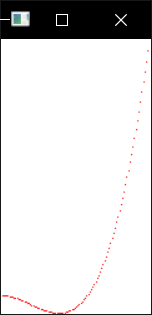
\includegraphics[width=0.3\linewidth]{wrong.png}
	}
	\quad\quad\quad
	\subfigure[Optimized]{
		\label{fig1.2}
		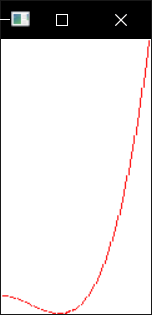
\includegraphics[width=0.3\linewidth]{result.png}
	}
	\caption{Result for $y= 0.0005x^3-0.03x^2+0.05x+100$}
	\label{fig1}
\end{figure}

%\bibliography{ref}{}
%\bibliographystyle{IEEEtran}
%========================================================================
\end{document}
